\documentclass[assd_tp3_main.tex]{subfiles}

\begin{document}

\section{Modulador delta}

\subsection{Introducci\'on}

El segundo conversor anal\'ogico/digital que se implement\'o fue un modulador delta. El mismo hace uso del principio de que, al muestrear una se\~nal a una frecuencia mucho mayor a la de Nyquist (oversampling), el valor de la misma no se altera significativamente entre muestra y muestra. Por lo tanto, codificando la diferencia entre una muestra y la siguiente, en lugar del valor de la muestra en s\'i, se puede ganar SQNR sin necesidad de incrementar el n\'umero de bits del ADC. El diagrama de bloques b\'asico de este conversor se observa en la figura \ref{fig:delta-bloques}.

\begin{figure}[htb]
	\centering
	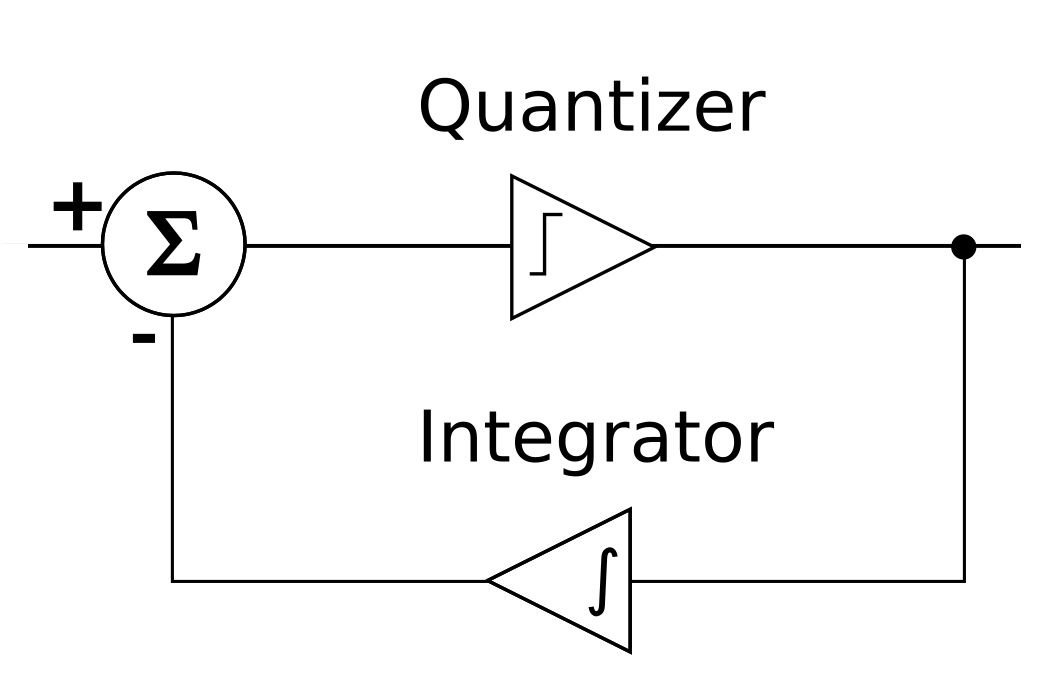
\includegraphics[width=0.6 \textwidth]
	{images/ej3/delta-bloques.png}
	\caption{Diagrama de bloques del modulador delta}
	\label{fig:delta-bloques}
\end{figure}

De esta manera, la salida digital del sistema indica si la se\~nal es mayor o menor a su \'ultimo valor, y de esta manera puede reconstruirse la se\~nal original utilizando un integrador (al igual que lo hace el realimentador).

La principal limitaci\'on que presenta este conversor es el tiempo de adquisici\'on, es decir, aqu\'el que se demora entre un cambio de full scale en la entrada, y que el mismo es observable en la salida. Dado que la salida s\'olo puede cambiar de a un bit por per\'iodo de muestreo, este tiempo limita la frecuencia m\'axima de entrada que se puede seguir con una cierta frecuencia de muestreo $f_s$. Llamamos $\Delta$ a la diferencia entre dos niveles l\'ogicos en la salida (un LSB), que en nuestro caso es:

\begin{equation}
	\Delta = \frac{5\mathrm{V}}{256-1} \sim 0.0196\mathrm{V}
	\label{eq:lsb}
\end{equation}

Luego, la condici\'on para que la salida pueda seguir a la entrada, es decir, que por cada per\'iodo de muestreo $T_s$, la salida no cambie m\'as de 1LSB, queda expresada como:

\begin{equation}
	\frac{dx}{dt} \leq \frac{\Delta}{2T_s}
\end{equation}

Si consideramos entradas senoidales de amplitud $V_p$ y frecuencia $f_0$, se obtiene entonces que:

\begin{equation}
	f_s \geq \frac{V_p}{\Delta} \cdot 4\pi f_0
	\label{eq:deriv}
\end{equation}

Considerando el valor obtenido en \ref{eq:lsb}, y que la tensi\'on pico m\'axima es $\nicefrac{5\mathrm{V}}{2} = 2.5\mathrm{V}$, se obtiene que:

\begin{equation}
	f_s \geq 510 \pi \cdot f_0 \simeq 1603 \cdot f_0
	\label{eq:f-sin}
\end{equation}

Dado que en este trabajo se utiliza $f_s \in [6$kHz, 45kHz], las senoidales m\'as r\'apidas que se puedan seguir ser\'an de entre 3.74Hz (para $f_s=6$kHz) y 28Hz (para $f_s=45$kHz).


\subsection{Implementaci\'on}

En este trabajo, la implementaci\'on utiliza la FPGA como integrador y un LM311 para realizar la resta y la cuantizaci\'on: su salida es $V_{CC}$ (un uno l\'ogico) cuando la entrada es mayor que la salida, y 0 (la tensi\'on de referencia, que a su vez representa un cero l\'ogico) cuando no. La FPGA recibe esta informaci\'on, e incrementa o decrementa un contador de 8 bits, dependiendo de si el comparador arroj\'o un 0 o un 1 respectivamente. Finalmente, el valor digital de este contador atraviesa un DAC0800 (con el mismo conexionado discutido en relaci\'on a la placa ADA), cuya salida se realimenta al LM311, cerrando as\'i el lazo de realimentaci\'on.

Dado a que se realiza una conversi\'on por per\'iodo de muestreo, a partir del valor instant\'aneo de la salida del comparador (con la frecuencia que selecciona el usuario, e implementado internamente en la FPGA), no es necesario utilizar un sample and hold en la entrada de este conversor. Sin embargo, por compatibilidad con el conexionado requerido para el conversor SAR (que s\'i lo requiere), se decidi\'o pasar la se\~nal por el mismo de todas maneras, cambiando s\'olo la se\~nal de control del mismo (determinada por la FPGA  para que se est\'e siempre en modo sample cuando el usuario indica que se debe trabajar en modo "modulador delta" (lo cual se implement\'o con jumpers que modificaban se\~nales que iban a la FPGA).


\subsection{Mediciones}

Para obtener la curva entrada-salida del conversor implementado, se realizaron mediciones de continua en todo el rango del conversor. Los resultados se observan en la figura \ref{fig:md-continua}.

\begin{figure}[!htb]
	\centering
	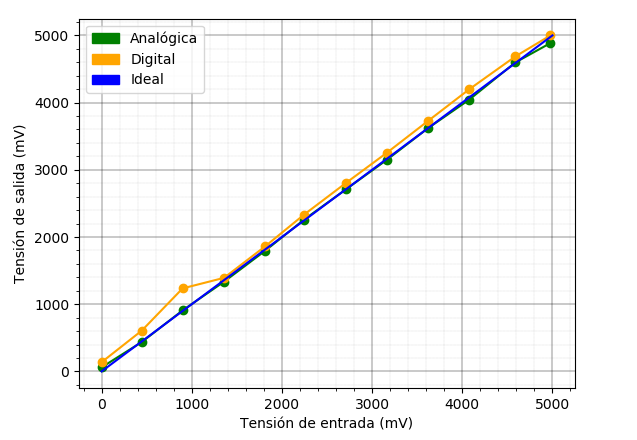
\includegraphics[width = \textwidth]
	{images/ej3/md-continua.png}
	\caption{Curva de entrada-salida del modulador delta, incluyendo su posterior conversi\'on a anal\'ogico y la curva ideal}
	\label{fig:md-continua}
\end{figure}

Se observa en la salida digital un peque\~no offset respecto de la entrada, pero tambi\'en respecto de su conversi\'on a anal\'ogica. Es razonable suponer, pues, que esto se debe a que el ruido inherente del sistema se manifestaba en los bits menos significativos, manteniendo los leds prendidos en todo momento, no porque estuviesen en 1, sino porque se encontraban oscilando.  Esto es, de hecho, exactamente lo que debe suceder en este conversor en la teor\'ia: como la salida no puede mantenerse constante, sino que debe subir o bajar un LSB en cada muestra, este es el comportamiento que se esperar\'ia.

Esto puede observarse m\'as claramente en la figura \ref{md-chiquita}. Aqu\'i, como la amplitud de la senoidal es de 25mV, que es apenas superior a los 20mV que representa el LSB, en los picos de la entrada, la salida oscila con 20mV de amplitud.


\begin{figure}[htb!]
	\centering
	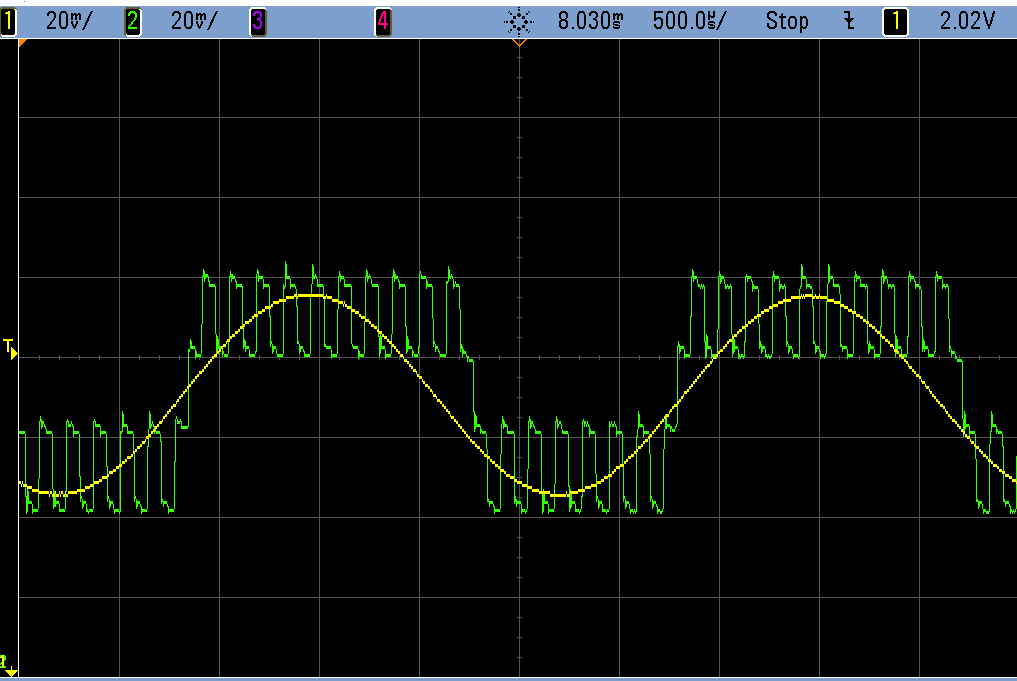
\includegraphics[width = 0.8\textwidth]
	{images/ej3/d__.png}
	\caption{Salida del modulador delta, con una entrada senoidal de 400Hz, 2V de offset, y 50m$\mathrm{V}_{PP}$ pico a pico}
	\label{fig:md-chiquita}
\end{figure}


Se observ\'o tambi\'en los efectos de reducir los bits activos en la salida. En la figura \ref{fig:md-bits}, resulta claro que una mayor contidad de bits conlleva m\'as precisi\'on, y m\'as niveles discretos a la salida.

\begin{figure}[htb!]
	\centering
	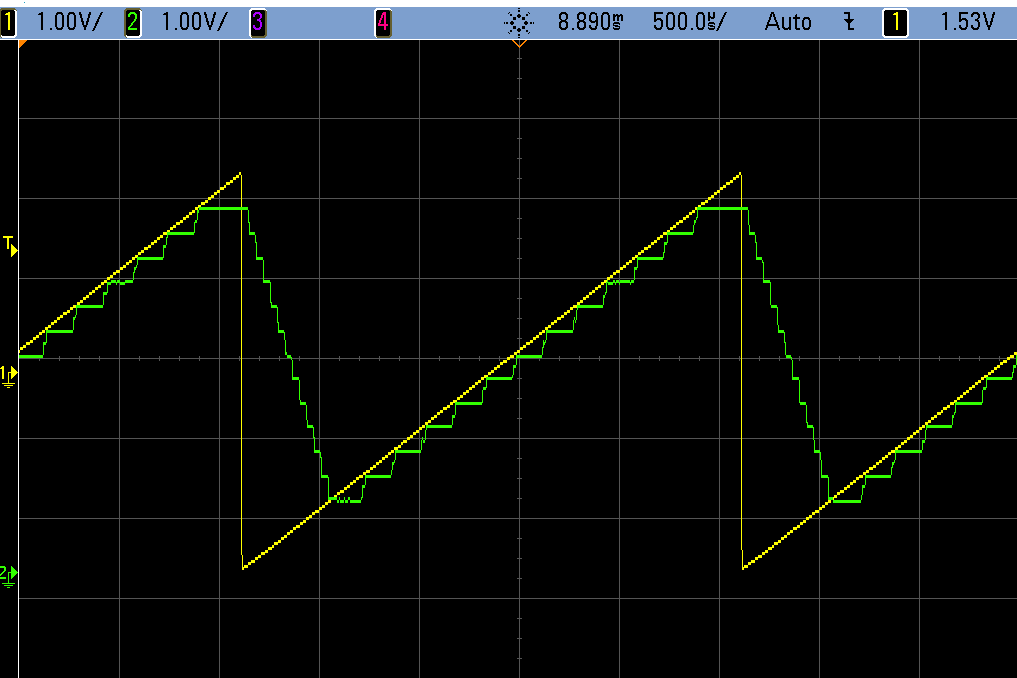
\includegraphics[width = 0.45\textwidth]
	{images/ej3/d_4.png}
	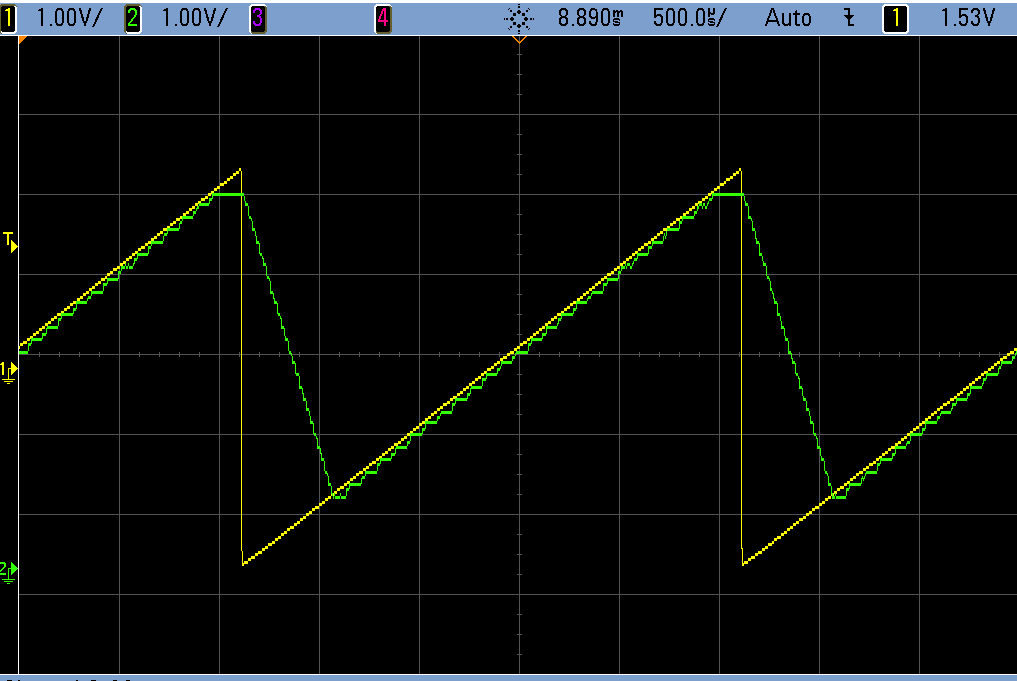
\includegraphics[width = 0.45\textwidth]
	{images/ej3/d_5.png}
	
	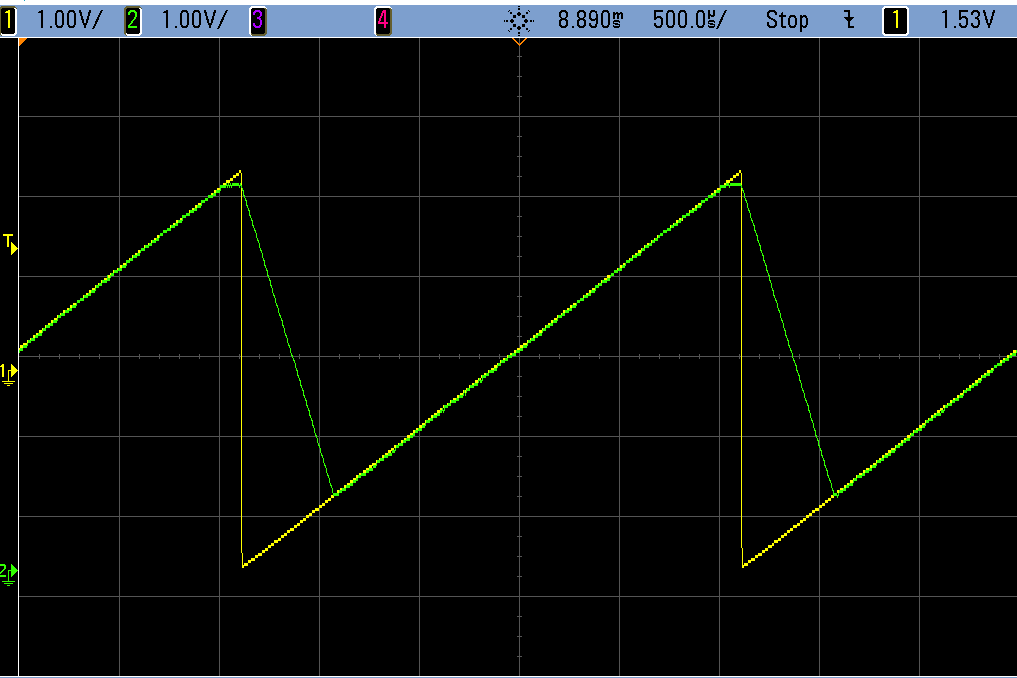
\includegraphics[width = 0.45\textwidth]
	{images/ej3/d_8.png}
	\caption{Salida del conversor con 4, 5 y 8 bits activos}
	\label{fig:md-bits}
\end{figure}

Algo que se esperar\'ia que ocurra, pero no se observa, es que el tiempo de adquisici\'on se reduzca, dado que al reducir N, aumenta $\Delta$, y con ello deber\'ia subir la frecuencia de sampleo m\'inima. Esto se debe a que, por consideraciones pr\'acticas, la anulaci\'on de bits se implement\'o s\'olo en la salida latcheada (que en este caso coincide siempre con la no latcheada, pero no as\'i para el SAR), con lo cual el loop de realimentaci\'on sigue funcionando en todo momento con 8 bits.

\end{document}